\documentclass[preview,border=0pt]{standalone}
\usepackage{tikz}
\usepackage[siunitx,RPvoltages]{circuitikz}
\begin{document}
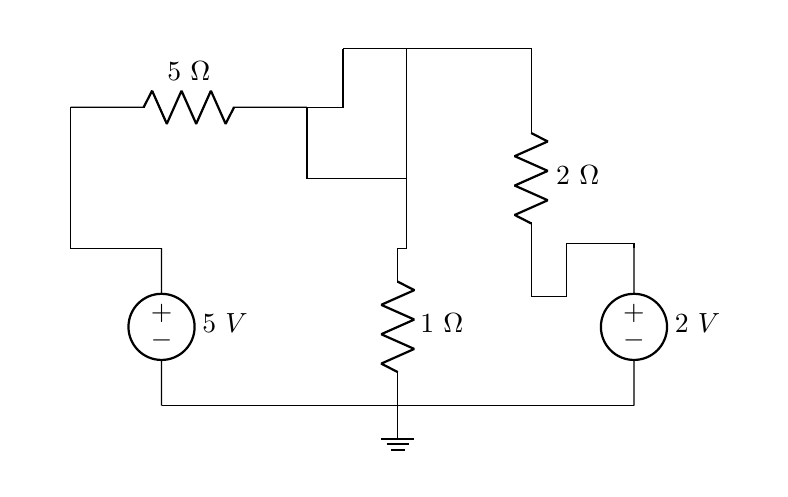
\begin{tikzpicture}
\useasboundingbox (3.3,5.2) rectangle (12.6,10.8);
\draw (5, 8) to[american voltage source, invert, l={$5 \ V$}] (5, 6);
\draw (11, 8) to[american voltage source, invert, l={$2 \ V$}] (11, 6);
\draw (3.847, 9.789) to[american resistor, l={$5 \ \Omega$}] (6.847, 9.789);
\draw (8, 8) to[american resistor, l={$1 \ \Omega$}] (8, 6);
\draw (9.695, 10.388) to[american resistor, l={$2 \ \Omega$}, label distance=0.06cm] (9.695, 7.388);
\draw (11, 6) |- (5, 6);
\node[ground] at (8, 6){};
\draw (6.847, 9.789) -| (7.305, 10.531);
\draw (7.305, 10.531) -| (8.109, 9.667);
\draw (8.109, 9.667) |- (7.185, 8.882);
\draw (8.109, 8.941) |- (8, 8);
\draw (6.847, 9.789) |- (7.185, 8.882);
\draw (9.695, 7.388) -| (10.147, 8.057) -| (11, 8);
\draw (3.847, 9.789) |- (5, 8);
\draw (9.695, 10.388) |- (8.109, 10.531);
\end{tikzpicture}
\end{document}
